\documentclass[a4paper,10pt]{article}

\usepackage[margin=1.5cm]{geometry}
\usepackage{url}
\usepackage[numbers]{natbib}
\usepackage[dvips]{graphicx}
\usepackage{amsmath}
\usepackage{float}
\usepackage{subfigure}
%% \usepackage{indentfirst}
\usepackage{listings}
\usepackage{color}
\usepackage{parcolumns}
\usepackage{setspace}
%% \usepackage{nopageno}
%% \usepackage{times}

%% \usepackage{blindtext}
%% \usepackage{draftwatermark}
%% \SetWatermarkText{\underline{C}onfidential}
%% \SetWatermarkScale{4}
%% \SetWatermarkColor[gray]{0.93}

%% \pagestyle{empty}

\def\CC{{C\nolinebreak[4]\hspace{-.05em}\raisebox{.4ex}{\tiny\bf ++}}}

\definecolor{lstgray}{gray}{0.95}

\lstset{ %
  language=C++,
  captionpos=b,
  basicstyle=\footnotesize,
  %% backgroundcolor=\color{lstgray},
  %% frame=single,
  frame=tb,
  %% frameround=tttt,
  tabsize=2,
  breaklines=true,
  breakatwhitespace=false,
  %% numbers=left,
  numbers=none,
  %% numbersep=5pt,
  %% numberstyle=\tiny\color{lstgray},
  xleftmargin=0pt,
  xrightmargin=0pt,
  morekeywords={in,out,inout,constexpr}
}

%% \lstset{frame=L, language=C++, basicstyle=\footnotesize\ttfamily, captionpos=b, keepspaces=true, columns=flexible}

\setlength{\columnsep}{8mm}
\setlength{\parindent}{4mm}
\renewcommand{\refname}{\Large{References}}


\title{Compile Time Differentiation Design}
\author{Dominic Jones}
\date{\today}

\begin{document}
\maketitle

\section{Specification}
Previous work on constructing the adjoint from a generated expression tree made use of destructors to trigger the evaluation. This approach works reasonably efficiently relative to its equivalent hand coded adjoint. The approach, however, had a fundamental limitation of not supporting nested function calls due to locally scoped variables prematurely triggering their adjoint evaluation upon destruction. Whilst the destructor approach, then, seemed to be the ideal solution to computing the adjoint, it also acted as the most significant hindrance to expanding functionality because of its implicit behaviour.

To resolve the nested function problem and to further improve the performance of the tool such that it could be on par with hand coded adjoint, a new approach was needed which did not rely on leveraging the destructors to trigger adjoint computation.

\section{Design}
To achieve on par performance with hand coded adjoint, the following constraints were followed:
\begin{enumerate}
\item work within the type system so the compiler can optimise as much as possible,
\item minimise the object size of the root node to prevent object copying dominating the execution time,
\item keep the memory layout well aligned, local, and always on the stack,
\item avoid \texttt{if} statements or conditional operators to manage evaluation,
\item aim to make the task of compiler optimisation nothing more than the micro-optimisation of inlining function calls,
\item avoid delegates or any form of call-back techniques.
\end{enumerate}

\section{Implementation}
For the illustration of implementation details, Figure \ref{fig:evaluate} and its equivalent code in Listing \ref{lst:evaluate} will be considered. Suppose the function in Listing \ref{lst:compute} was required to be differentiated. The aim of the differentiation tool is such that by providing the appropriate \texttt{Mode} type and including the header file of the tool, the primal, tangent or adjoint function would be compiled.\newline
\begin{lstlisting}[caption={Nested function calls must propagate their expression trees.}, label=lst:compute]
#include <exprlist.h>
template<class Mode>
void compute()
{
  Terminal<Mode, A const> a;
  Terminal<Mode, B const> b;
  Terminal<Mode, R> r;
  r = evaluate(evaluate(a, b), evaluate(b, a));
}
\end{lstlisting}

\begin{minipage}{\linewidth}
  \centering
  \begin{minipage}{0.45\linewidth}
    \begin{figure}[H]
      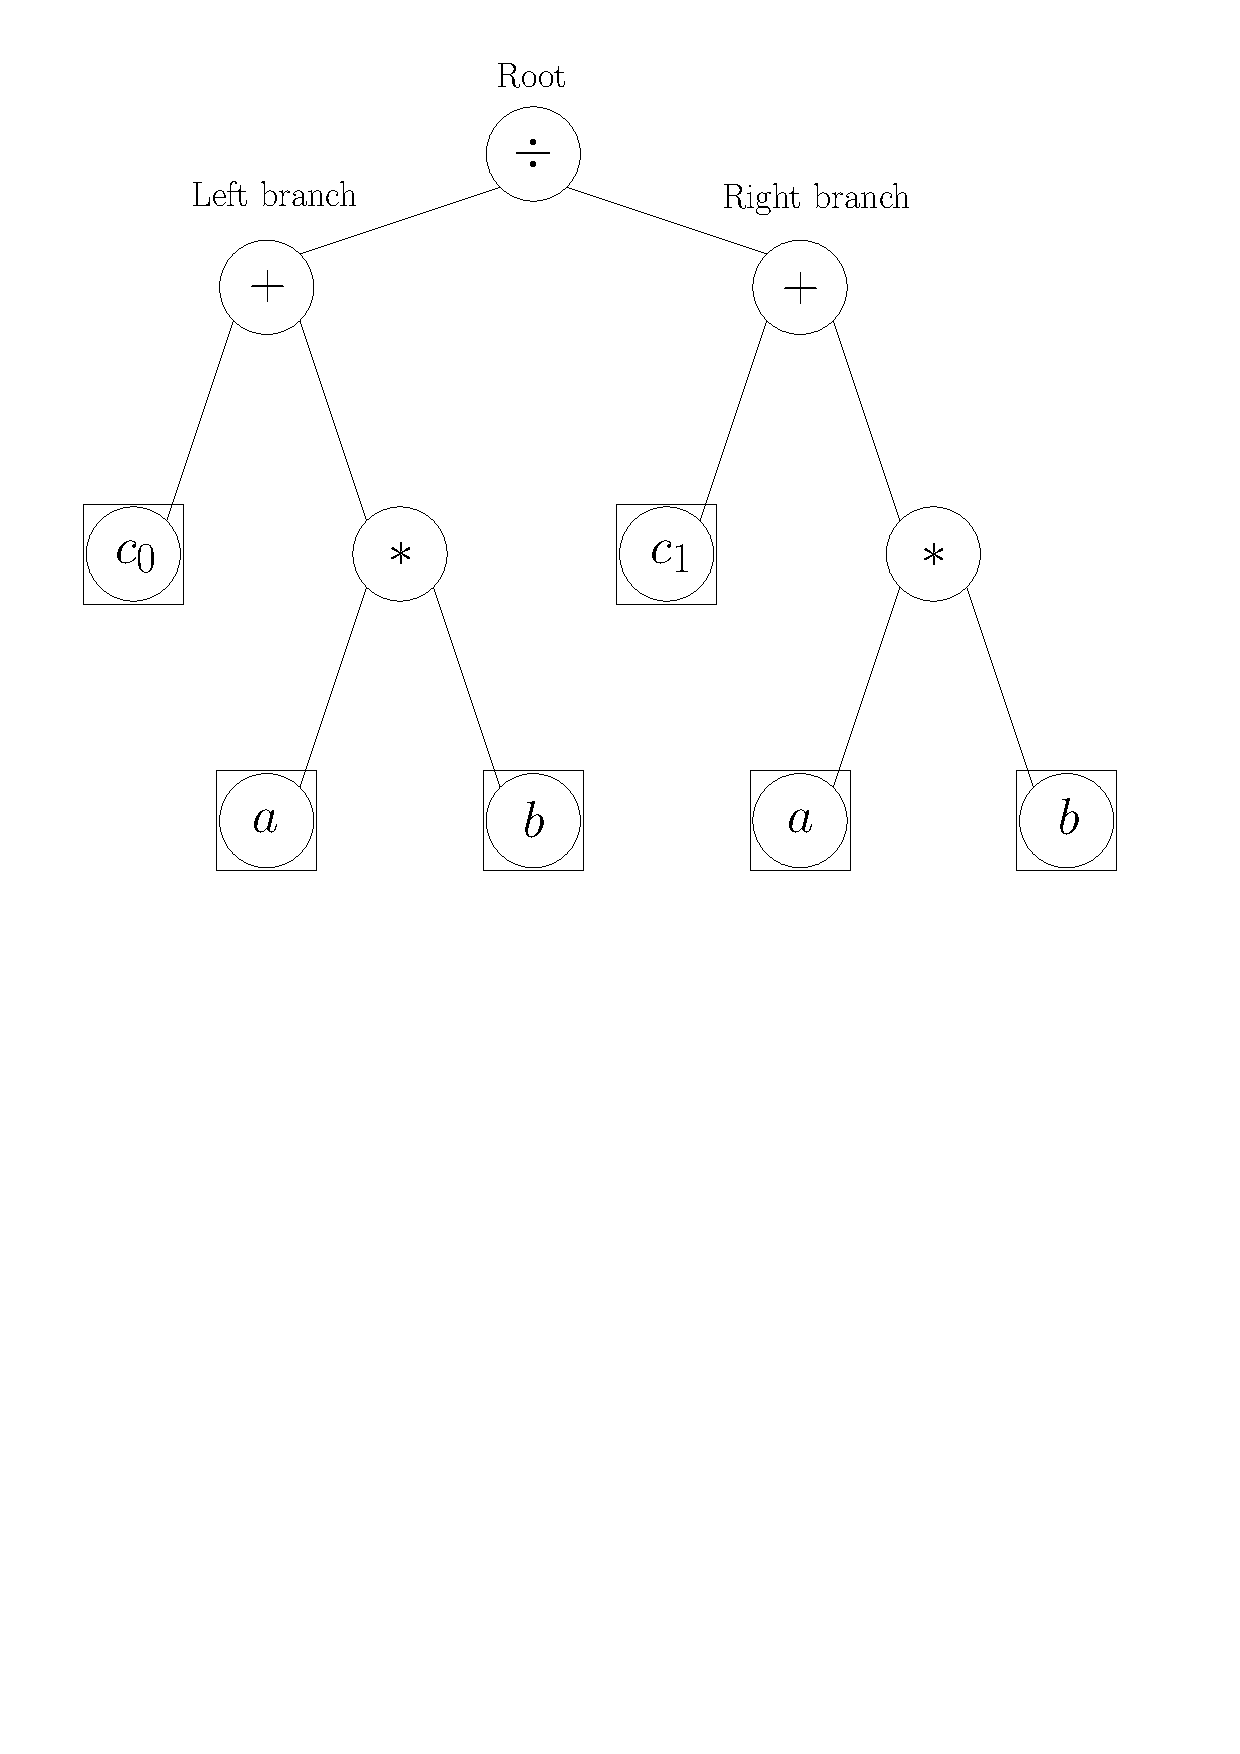
\includegraphics[width=\linewidth]{fig_exprtree}
      \caption{Duplicate branch? Impossible to tell given only the types.}
      \label{fig:evaluate}
    \end{figure}
  \end{minipage}
  \hspace{0.05\linewidth}
  \begin{minipage}{0.45\linewidth}
\begin{lstlisting}[caption={\texttt{lb} and \texttt{rb} have the same type but do not represent the same expression.}, label=lst:evaluate]
template<class TA, class TB>
auto evaluate(TA a, TB b)
{
  auto c0 = 3;
  auto c1 = 4;
  auto ab = a * b;
  auto lb = c0 + ab;
  auto rb = c1 + ab;
  return lb / rb;
}
\end{lstlisting}
  \end{minipage}
\end{minipage}

\subsection{Building the tree}
To evaluate the root in any mode, the expression tree must
\begin{enumerate}
\item build up the full type of the expression
\item capture the addresses of the active terminal nodes
\item capture the values of the passive terminal nodes
\end{enumerate}
Typical expression template tools will store the intermediate state at each node, though this is not necessary. Intermediate state is only required when evalution of the root is triggered, and so any optional allocation can be delayed until then.

\subsubsection{Expression list}
Building up of the expression type is straight forward: by using \texttt{auto} for the variable and return types, each new expression nests the types of its arguments. One problem exists with this, however. The expression type is nothing more than a type, and therefore conveys no information about whether or not two or more identical types found in the full expression type are semantically the same thing. Figure \ref{fig:evaluate} demonstrates the problem: how can duplicate subexpressions be identified in order to avoid duplicate evaluation? With only type information it is not possible since the values may be different. Since comparing memory addresses of subnodes of same type would violate the design requirements (causing excessive run-time overhead), the alternative was to somehow encode into the type the identity of the subexpression such that duplicate subexpression matching can be correctly performed.\newline
Listing \ref{lst:unique} offers a solution, though using it requires decorating passive values with the preproccessor function (i.e. \verb$auto c0 = UQ(3);$). Furthermore, template functions are needed to evaluate mathematical operations performed on passive values decorated with the unique type and return new unique types with the resulting value.
\begin{lstlisting}[caption={\texttt{\_\_COUNTER\_\_} offers a non-standard way to distinguish variables.}, label=lst:unique]
// simple class to identify unique types
template<std::size_t ID, class T> struct Unique { T value; };

// hide __COUNTER__ behind macro
#define UQ(value) Unique<__COUNTER__, decltype(value)>{value}
\end{lstlisting}

Whilst building the expression type poses no difficulties, building the unique list of operations does. This task is a type transformation, converting the expression tree as it is being built. Considering Figure \ref{fig:evaluate}, its expression type would like that of Listing \ref{lst:evaluate-type}, whereas the expression list would be like that of Listing \ref{lst:evaluate-type-list}: a list of lists order according to depth, with each depth containing unique types.\newline
\begin{minipage}{\linewidth}
  \centering
  \begin{minipage}{0.45\linewidth}
\begin{lstlisting}[caption={Expression type of Figure \ref{fig:evaluate}.}, label=lst:evaluate-type]
Binary<Div,
  Binary<Add,
    Unique<0, double>,
    Binary<Mul, A, B> >
  Binary<Add,
    Unique<1, double>,
    Binary<Mul, A, B> > >
\end{lstlisting}
  \end{minipage}
  \hspace{0.05\linewidth}
  \begin{minipage}{0.45\linewidth}
    \begin{lstlisting}[caption={Expression type list of Figure \ref{fig:evaluate}.}, label=lst:evaluate-type-list]
// template<class... Ts> struct list {};
list<
  list<A, B>,
  list<Binary<Mul, A, B> >,
  list<Binary<Add, Unique<0, double>, ...>,
       Binary<Add, Unique<1, double>, ...> >,
  list<Binary<Div, ..., ...> > >
\end{lstlisting}
  \end{minipage}
\end{minipage}

A problem not encountered in this simple case is where one subexpression is deeper than the other. Merging of the two sublists can only be performed if they are the same length. To remedy this problem, both sublists are first resized to the larger of the two, and padded with empty nested lists if required.

\subsubsection{Active terminals}
Capturing the addresses of the active terminal nodes efficiently is non-trivial as both types and data are involved. Considering again Figure \ref{fig:evaluate}, the terminal nodes are repeated in the left and right branches. This duplication needs to be avoided and so at every node which is not a unary operation, a merge operation of the addresses must be performed. Ordinarily, the number of unique active terminals will be small regardless of the size of the expression tree, so little benefit is gained from having a highly efficient implementation of the merge operation.

\subsubsection{Passive terminals}
Capturing the values of the passive terminal nodes is essentially the same task as capturing the addresses of the active terminals. The only significant difference here is that the efficiency of the merge operation does become a factor as the number of values typically scales with the size of the tree. For both this and the merging of the active terminals the same function is used. In Listing \ref{lst:merge} two sets are merged: \texttt{s1} and \texttt{s2}. Since at least all of one of the sets will be included in the new set, the bigger of the sets is selected immediately. The next task is to find any of the members of the smaller set in the larger set. If there are any that are not found, add them to the new set. This search operation is presently implemented naively: each memeber of \texttt{s2} is searched for in \texttt{s1}. However, this could be improved: given that elements are always in the same order (in this case \texttt{char} is always followed by \texttt{bool}) and elements are unique, the search space in \texttt{s2} can be reduced after each elemental search of \texttt{s1}. So, for \texttt{char} in \texttt{s1}, all elements in \texttt{s2} must be searched, but for \texttt{bool} in \texttt{s1} only the third and fourth elements in \texttt{s2} must be searched, and finally, for \texttt{double} in \texttt{s1}, no search needs to be performed since the \texttt{bool} found in the previous search was already at the upper bound of \texttt{s2}.\newline
\begin{lstlisting}[caption={A simplified example of merging two sets.}, label=lst:merge]
  std::tuple<char, bool, double> s1{'c', true, 5.6};
  std::tuple<int, char, float, bool> s2{2, 'c', 3.4, true};

  // std::tuple<char, bool, double, int, float>
  auto s3 = merge(s1, s2);
\end{lstlisting}

\subsection{Evaluating the list}
Building the expression list accounts for much less than half of the compiler work; the bulk of the compilation is building the index lists for the intermediate data and passive values and secondly for looping over the node operations in order for the primal then in reverse order for the adjoint.

\subsubsection{Indexing the expression list}
For unary, binary and ternary nodes, their left, middle and right data indices are required. Given the list from Listing \ref{lst:evaluate-type-list}, the index lists would be:\newline
\begin{lstlisting}[caption={Generating the left, middle and right indices.}, label=lst:expression-indices]
// from:
list<A, B, Binary<Mul, ...>, Binary<Add, Unique<0, double>, ...>, Binary<Add, Unique<1, double>, ...>, Binary<Div, ...> >

// construct: (ic -> std::integral_constant)
list<ic<6>, ic<6>, ic<0>, ic<6>, ic<6>, ic<3> > // left indices
list<ic<6>, ic<6>, ic<1>, ic<2>, ic<2>, ic<4> > // middle indices
list<ic<6>, ic<6>, ic<6>, ic<6>, ic<6>, ic<6> > // right indices
\end{lstlisting}
Since \texttt{A} and \texttt{B} have no subexpressions, the left, middle and right indices are always set to the out of range value (i.e. the size of the expression list after flattening it), and likewise for the passive terminals. Also, since there are no ternary expressions in the example then all the right indices are out of range. Implementing the function to generate these index lists is fairly involved though efficient: for any given node its subnodes can be deduced and from them their depth. Since the expression list is depth ordered then only the elements in the specific depth need to be searched.

\subsubsection{Indexing the passive values}
Indexing the passive value data follows the same first step as indexing the subexpressions, but there is an additional step that must also be performed. Again, using the same example, the required index list would be:\newline
\begin{lstlisting}[caption={Generating the passive value mapping.}, label=lst:passive-indices]
// from:
list<A, B, Binary<Mul, ...>, Binary<Add, Unique<0, double>, ...>, Binary<Add, Unique<1, double>, ...>, Binary<Div, ...> >

// construct:
list<ic<3>, ic<4> > // indices (step 1)
list<ic<2>, ic<2>, ic<2>, ic<0>, ic<1>, ic<2> > // dual of 'indices' (step 2)
\end{lstlisting}

\subsubsection{Evaluating the operations}
Evaluation of the full expression list is performed by recursively stepping through each node in the list, first in order to compute the primal, and then in reverse order to compute the adjoint. Intermedate data both for the primal and adjoint is stored in \texttt{std::tuple}s, so accessing elemental values requires using \texttt{std::get}. This has turned out to be very expensive to compile for large expression trees, compared to if the data was simply stored in \texttt{std::arrays}s and the subscript operator used to access values.

One possible improvement to minimise the compilation time due to the use \texttt{std::get} for very large lists is to evaluate the full expression list as a list of lists ordered by depth. This would mean that \texttt{std::get} is operating over a much smaller range and so should reduce compile time despite double indirection being required.

\section{Further work}
\subsubsection{Multiple assignments}
The present method only efficiently supports one assignment because it is at the point of assignment that all the computation is performed therefore having more than one assignment will almost inevitably mean duplicate evaluations being performed. There is no obvious work-around to this problem. Whatever the solution though, somehow it must bring together the different output terms so as to make them visible with a single assignment operation. Furthermore, probably some sort of checkpointing on the roots of the results would be required.

Finally, though it would be very contrived, some way of bringing the various roots into a single root and the evaluating like normal on that single root would work. This might mean adding a special operator which can work as a mechanism to seed the result roots and also join it to the the final root.\newline
\begin{lstlisting}[caption={Combining multiple roots into one.}, label=lst:multiple-roots]
evaluate2(A a, B b, R1 &r1, R2 &r2)
{
  auto t1 = a + b;
  auto t2 = (a * b) / t1;

  // cache adjoint result seeding values
  auto expr_r1 = assign_result(r1, t1);
  auto expr_r2 = assign_result(r2, t2);

  // combine subexpressions (using addition)
  // and evaluate
  evaluate_tree(expr_r1, expr_r2);
}
\end{lstlisting}

\subsubsection{\texttt{std::get} alternative}
The standard library implementation for accessing elemental data in a \texttt{std::tuple} incurs a relatively long compile time and performs relatively poorly to a homogeneous container, such as \texttt{std::array}, even when the types in the tuple are identical. Efforts to remedy the poor compilation time have been tried by implementing an alternative hetrogeneous container, along with accessor functions. This alternative implementation remedied the compilation time, effectively halving it for large tests, but inlined poorly, resulting in relatively slow run times.

Boost Hana offers its own tuple implementation which claims to have both good compile time and run time performance, though it has not been tested in this work.

\subsubsection{Merge operation}
The merging of the passive values for a binary node presently incurs the single biggest run time performance loss. This is highlighted by comparing the run time of a large case with the using the present constructor and with the default constructor. Clearly, in the second case the results will be meaningless, but the test highlights that the constructor operation is not getting inlined. The reason for this is likely to be due to the amount of compilation work required to implement the constructor. As noted above, there are improvements that could be made to trim down the amount of unrolling required for the merge operation. This task, though difficult, would probably yield the single biggest benefit to the methodology.


\subsubsection{Recursive evaluation}
The operation list is iterated naively using recursion for both primal and adjoint evaluation, and its compilation accounts for a major proportion of the overall time. Other techniques exist for iterating over lists, such as using multiple inheritance or the function signature matching technique. These may yield meaningful compilation time improvements, though none has been tested.

\end{document}
